\begin{figure}[t!]
% http://en.wikibooks.org/wiki/LaTeX/Floats,_Figures_and_Captions
% http://tex.stackexchange.com/questions/119984/subfigures-side-by-side-with-captions
%\usepackage{caption}     %% loads OK, but not needed neither subfigure nor subcaption
                          %% work under Tufte-book template
%\usepackage{subfigure}   %% This package loads without errors, however 
                          %% \begin{subfigure}[t]{0.49\textwidth} DOES NOT WORK!
%\usepackage{subcaption}  %% ! Package caption Error: The `subcaption' package does not work 
                          %%   correctly in compatibility mode.
\centering
\vspace*{-0ex}% removes white space at the top

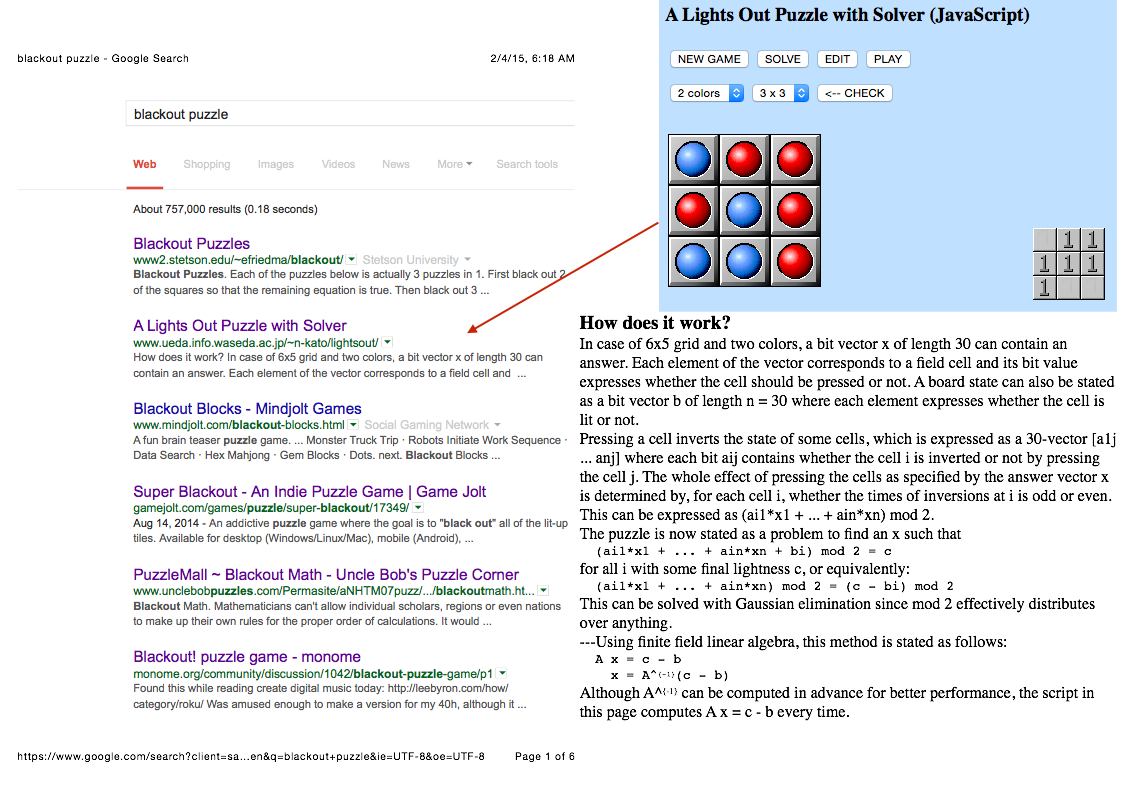
\includegraphics[width=0.99\textwidth]{fg-key-blackp-descr-a}
\vspace*{1ex}% removes white space for the next figure 
\\
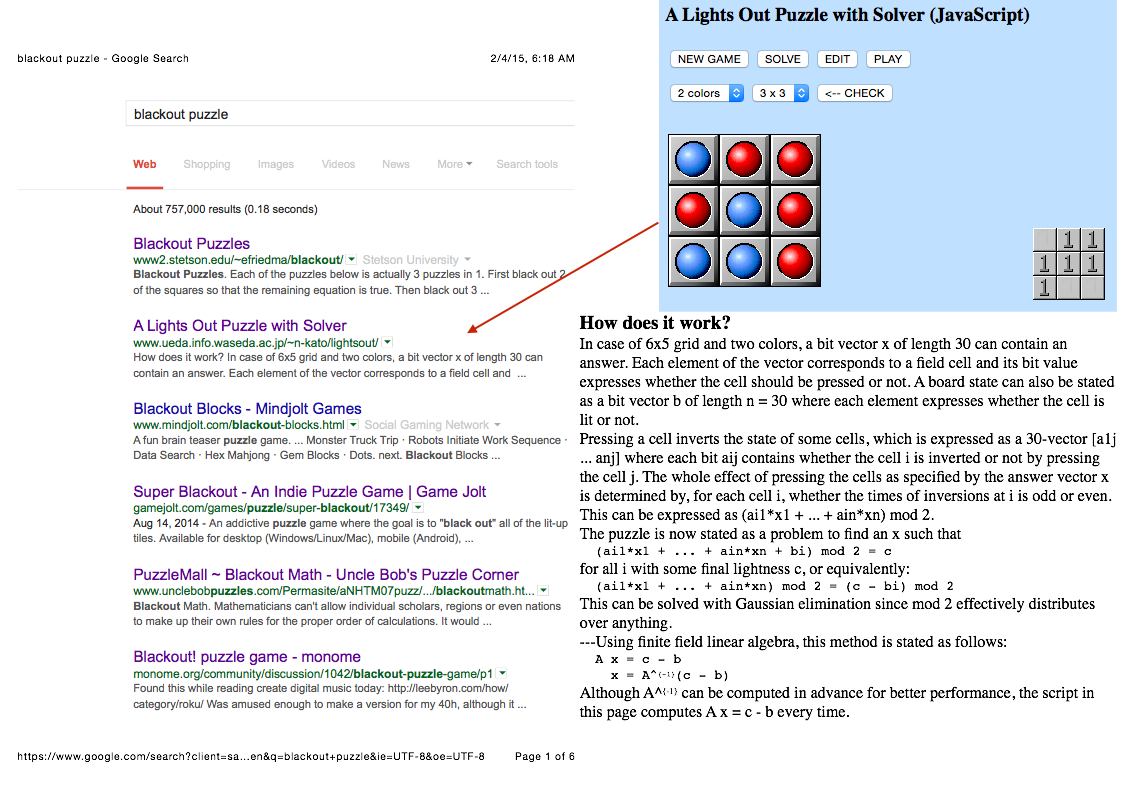
\includegraphics[width=0.99\textwidth]{fg-key-blackp-descr-a}
\vspace*{1ex}% removes white space for the next figure 
\\
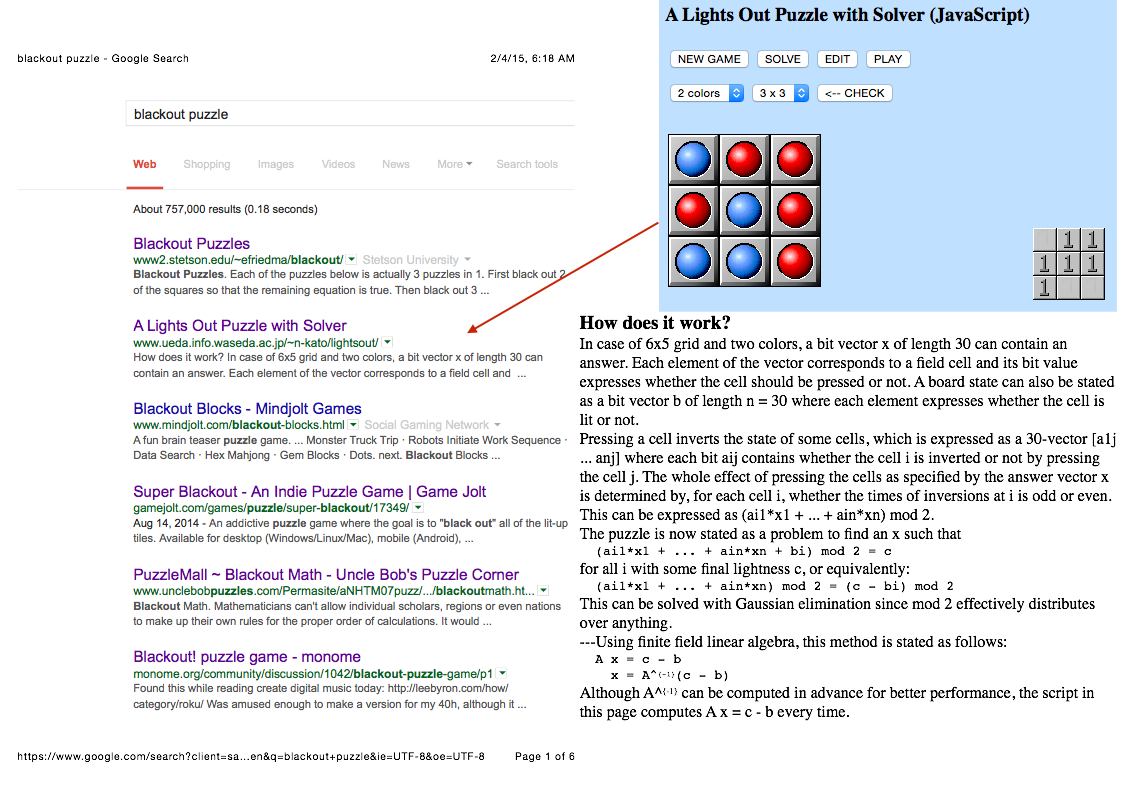
\includegraphics[width=0.99\textwidth]{fg-key-blackp-descr-a}
\vspace*{1ex}% removes white space for the next figure 
%
% https://github.com/fbrglez/gitPublic/tree/master/xProj499-Sp15
\caption[From the file fg-key-blackp-normal-3-figures.tex]
{From the file fg-key-blackp-portrait-3-figures.tex {\em borrowed from} {\tt Lib-OPUS2-ebook-CSC499-Sp15-2015-Brglez}.
{\bf NOTE: both `verb' and `cite' commands seem disabled under `figure environment'!}
Also, the portrait of 3 plots from Keynote are larger than the 3 plots from R in portrait format,
see Figure~\ref{fg-R-labs-portrait-3-figures}.
Then,
(a) 
it may not be possible to create (a) in this file with \LaTeX ... may need to create it in Keynote;
%
(b)
it may not be possible to create (b) in this file with \LaTeX ... may need to create it in Keynote;
%
(c)
it may not be possible to create (c) in this file with \LaTeX ... may need to create it in Keynote.
}
\label{fg-key-blackp-normal-3-figures}
\end{figure}


